\section{Evaluation}

To evaluate a system, it is necessary to have access to metrics to quantify its performance.In the case of machine learning algorithms, the most important metric is Error.

\subsection{True vs Empirical Error}
The error that we can observe, the \textbf{Empirical Error}, is the one related to the training set available to us, and it can vary from set to set. The \textbf{Actual Error}, on the other hand, is generally unknown to us and is the classification error of all possible examples.

\subsubsection{Example}
\begin{itemize}
    \item[\textcolor{green!50!black}{\textbullet}] Correctly classified: $f(x) = h(x)$
    \item[\textcolor{red}{\textbullet}] Misclassified: $f(x) \not= h(x)$
\end{itemize}
\begin{center}
    \begin{tabular}{c}
        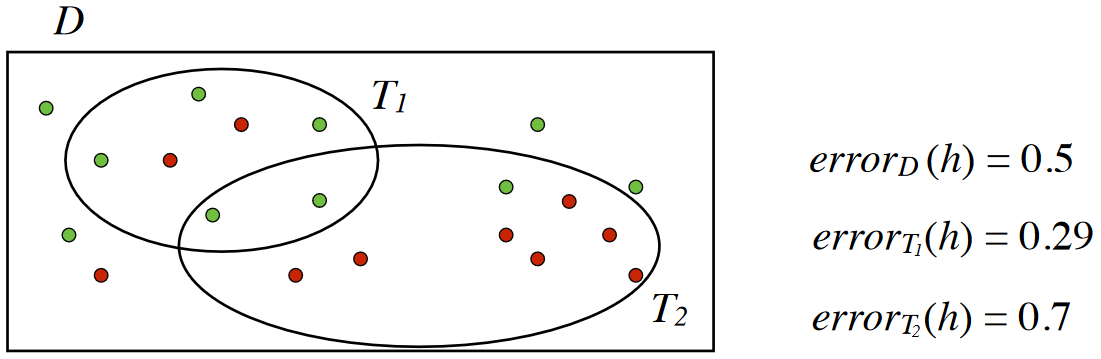
\includegraphics[width=0.8\textwidth]{images/Error.png}
    \end{tabular}
\end{center}
Depending on the training set the model may have too much bias or have too much variance.  In the image the $T_1$ set of examples leads the model to have too much optimistic bias, the $T_2$ set on the contrary has too much variance and therefore any corrections are likely to be detrimental to the model because they will increase the bias or variance in the wrong directions.  To improve our assessment of model performance it is important to make sure that the \textbf{Empirical Error} is as close as possible to the \textbf{True Error}.

\subsection{Model Selection}

\subsubsection{Hold-out}
\textbf{Hold-out} is the procedure that, once a training data set is defined, splits it into several subsets and one of those will be the set used to evaluate the model, also called the validation set.
\begin{itemize}
    \item A classifier/regressor will then be trained on the training set data except those in the validation set and another, used to evaluate the performance of the model, called the test set.
    \item Usually the size of the training + validation sets should be larger than the test set, for example 70\%, 15\% and 15\% respectively.
    \item The validation and test sets, which are not used for training, are used to be able to verify the model on data it has never seen.
    \item In this way, however, the validation and test data are useless for training.
\end{itemize}
\newpage
\subsubsection{K-fold Cross Validation}
The most common method of making them useful is called \textbf{K-fold Cross Validation}, in which:
\begin{enumerate}
    \item The dataset is divided into $k$ equal partitions, the algorithm uses $k-1$ of them for training and the remaining partition for validation;
    \item This procedure is performed $k$ times, leaving a different partition out of the training set each time;
    \item Finally, the various results obtained are averaged to calculate the overall performance of the model;
    \item At this point a final evaluation of the resulting model can be made using the test set, which was not used within the cross validation, to avoid overestimating performance.
\end{enumerate}       

\subsubsection{Leave-one-out}
A special case of k-fold cross validation, called \textbf{Leave-one-out}, is when the number of partitions chosen matches the number of data within the training set, and thus at each iteration the training set will contain all but one of the available data.
The purpose of cross validation is therefore to try to converge, as $k$ increases, the average error they compute to the true error. But of course as $k$ increases, the computational cost also increases since you have to redo $k$ times the training so it is usually used with a relatively small $k$, usually $10$.

\subsection{Metrics}
Evaluation metrics define how the goodness-of-fit of the model is evaluated.  We consider several different metrics per classification task, starting with an example:
\begin{center}
    \begin{tabular}{c}
        \\ 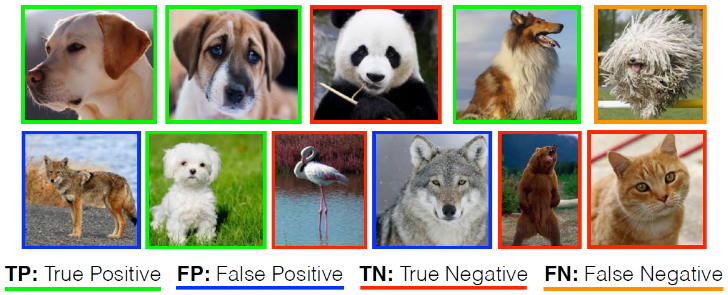
\includegraphics[width=0.8\textwidth]{images/Metrics1.png} \\ \\
    \end{tabular}
\end{center}
Evaluation metrics define how the goodness-of-fit of the model is evaluated.  We consider several different metrics per classification task, starting with an example:
\begin{center}
    \begin{tabular}{c}
        \\ 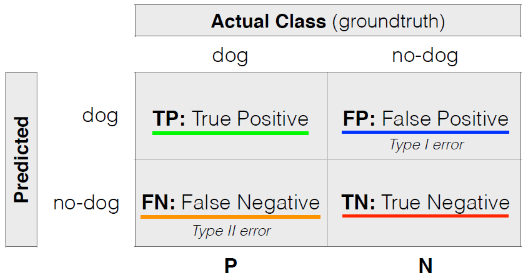
\includegraphics[width=0.6\textwidth]{images/Metrics2.png} \\ \\
    \end{tabular}
\end{center}
Using this information we then see various metrics for a model:
\begin{itemize}
    \item \textbf{Accuracy:} calculate how accurate it is
    \begin{equation} \tag{Accuracy}
        \frac{TP + TN}{P + N} = \frac{\text{all correct}}{\text{all instances}} = \frac{8}{11} \approx 0.73
    \end{equation}
    \item \textbf{Precision:} calculate how precise it is
    \begin{equation} \tag{Precision}
        \frac{TP}{TP + FP} = \frac{TP}{\text{all predicted}} = \frac{4}{6} \approx 0.67
    \end{equation}
    \item \textbf{Recall:} calculate how well it can predict
    \begin{equation} \tag{Recall}
        \text{sensitivity} = TPR = \frac{TP}{TP + FN} = \frac{TP}{\text{all actual}} = \frac{4}{5} = 0.80
    \end{equation}
    \item \textbf{False Positive Rate:} calculate how many of the incorrect predictions it makes
    \begin{equation} \tag{FPR}
        \frac{FP}{FP + TN} = \frac{FP}{\text{all incorrect}} = \frac{2}{6} \approx 0.33
    \end{equation}
    \item \textbf{F1-Score:} the harmonic mean of precision and recall
    \begin{equation} \tag{F1-Score}
        2 \cdot \frac{\text{Precision} \cdot \text{Recall}}{\text{Precision} + \text{Recall}}
    \end{equation}
    \item \textbf{Average Precision (AP):} combines recall and precision for a ranked list
    \begin{equation} \tag{AP}
        \frac{\sum^n_{k=1} P(k) \cdot R(k)}{\text{all actual}}
    \end{equation}
    \item \textbf{mean Average Precision (mAP):} the average of all AP values
    \begin{equation} \tag{mAP}
        \frac{1}{Q} \cdot \sum^Q_{q=1} AP(q)
    \end{equation}
\end{itemize}

\newpage